\section{Measuring Reflectances of Optical Elements} 
\label{sec:reflectances}
In this section, we describe the procedure used to measure the reflectances of the LSSTCam optical elements (i.e., Detector, Filter, L1, L2, L3) using the strength of optical ghosts produced in test data collected with the Collimated Beam Projector (CBP) \citep{2016SPIE.9906E..0OI}. 
This serves as a verification of the reflectances used in the \texttt{Batoid} simulations in the previous sections, which in turn also validates the reflectances used in systems engineering simulations.

\subsection{Optical Ghosts and Reflectances}
\label{sec:reflectance_theory}
To form a first-order ghost, a ray of light must be reflected successively by two optical elements (higher-order ghosts also exist, but are highly suppressed, as they require four or more successive reflections).
The probability that a ray contributes to the flux of the ghost is $P_{AB} = R_A R_B$, where $R_A$ and $R_B$ are the reflectances of the optical elements A and B, respectively.
The flux of an optical ghost can therefore be related to the flux of the source through $P_{AB}$, as shown in Eq.~\ref{eq:ghost_flux_prob}, where $f_{A, B}$ is the flux of the ghost and $f_{\rm src}$ is the total incident flux of the astronomical source (i.e., bright star).

\begin{equation}
\label{eq:ghost_flux_prob}
f_{A,B} = R_A R_B f_{\rm src}
\end{equation}

\noindent Measurements of $f_{A,B}$ and $f_{\rm src}$ allow a determination of the combined reflectances of the optical elements involved in the production of the ghost.

Considering all ghosts produced by different combinations of optical elements leads to a set of coupled equations.
A subset of these equations, limited to ghosts arising from a reflection off of a filter surface (F1 or F2) and either the  Detectors (D) or a surface of Lens 3 (L31 or L32), is shown in Eq.~\ref{eq:coupled_eqs}.

\begin{equation}
\label{eq:coupled_eqs}
\begin{aligned}
f_{F1 , F2} &= R_{F1} R_{F2} f_{\rm src} \\
f_{L{32} , F1} &= R_{L{32}} R_{F1} f_{\rm src} \\
f_{L{32} , F2} &= R_{L{32}} R_{F2} f_{\rm src} \\
f_{L{31} , F1} &= R_{L{31}} R_{F1} f_{\rm src} \\
f_{L{31} , F2} &= R_{L{31}} R_{F2} f_{\rm src} \\
f_{D , F1} &= R_{D} R_{F1} f_{\rm src} \\
f_{D , F2} &= R_{D} R_{F2} f_{\rm src}.
\end{aligned}
\end{equation}
\noindent This system of equations can be linearized in log-space as follows:
\begin{equation}
    \label{eq:log-coupled-eqs}
    \log\left(\frac{f_{A,B}}{f_{\rm src}}\right) = \log R_A + \log R_B.
\end{equation}
With a redefinition of variables $x_A \equiv \log R_A$ and $b_{A,B} \equiv \log \left(\frac{f_{A,B}}{f_{\rm src}}\right)$, the system of equations in log-space can be written as a matrix problem $A\vec{x} = \vec{b}$ (expanded form in Eq.~\ref{eq:reflectance_matrix}), where the reflectances can be solved for with least squares by inverting the matrix $A$. 
Here, the vector $\vec{x}$ contains the log reflectances and the vector $\vec{b}$ contains the ghost fluxes.
This system can thus be solved independently of knowing the source flux.
\begin{equation}
\label{eq:reflectance_matrix}
\begin{pmatrix}
1 & 1 & 0 & 0 & 0 & \dots \\
0 & 0 & 0 & 0 & 0 & \\
1 & 0 & 0 & 0 & 0 &  \\
0 & 1 & 0 & 0 & 0 & \dots \\
\vdots & & & & \vdots & \ddots \\
\end{pmatrix} \, 
\begin{pmatrix}
x_{F_1} \\
x_{F_2} \\
x_{L_{11}} \\
x_{L_{12}} \\
\vdots \\
\end{pmatrix}\,\,
=
\begin{pmatrix}
b_{F_1 , F_2} \\
b_{L_{32} , L_{31}} \\
b_{L_{32} , F_1} \\
b_{L_{32} , F_2} \\
\vdots \\
\end{pmatrix}
\end{equation}

\subsection{Measuring Ghost Fluxes}
\subsubsection{Data}
\begin{figure}[h!]
    \centering
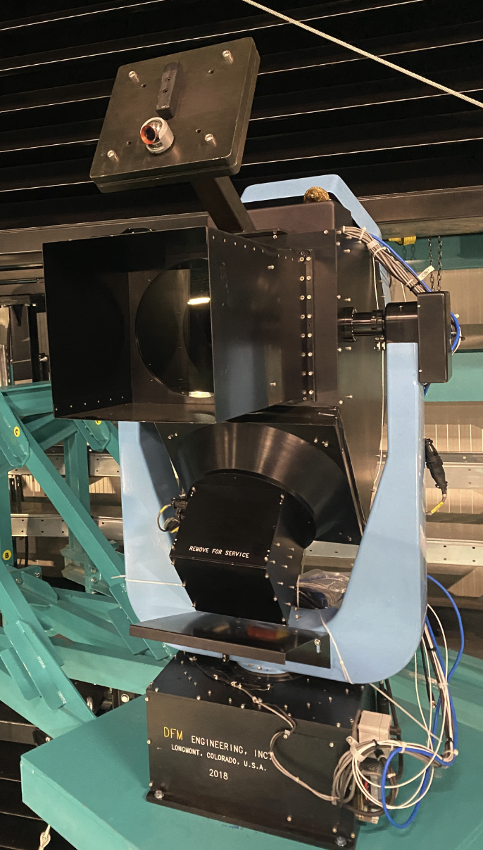
\includegraphics[width=0.2\textwidth]
{figures/CBP_dome_front.png}
    \caption{An image of the Collimated Beam Projector (CBP) from \cite{SITCOMTN-152}.} 
    \label{fig:cbp}
\end{figure}

The Collimated Beam Projector (CBP) is a repurposed 30\,cm Schmidt telescope that has been fitted with a laser and mounted to the Rubin dome. It is located approximately 12.5\,m from the Telescope Mount Assembly (TMA) at a height of approximately 14\,m.
The CBP projects a
monochromatic point-like source in a parallel beam onto the primary mirror (M1), thereby allowing to produce an artificial
light source mimicking the behaviour of a star.
Note that the CBP doesn't illuminate the entirety of M1 as a star would, changing the morphology of the observed ghosts.

\begin{figure}[h!]
  \centering

  \begin{subfigure}[t]{0.45\textwidth}
    \centering
    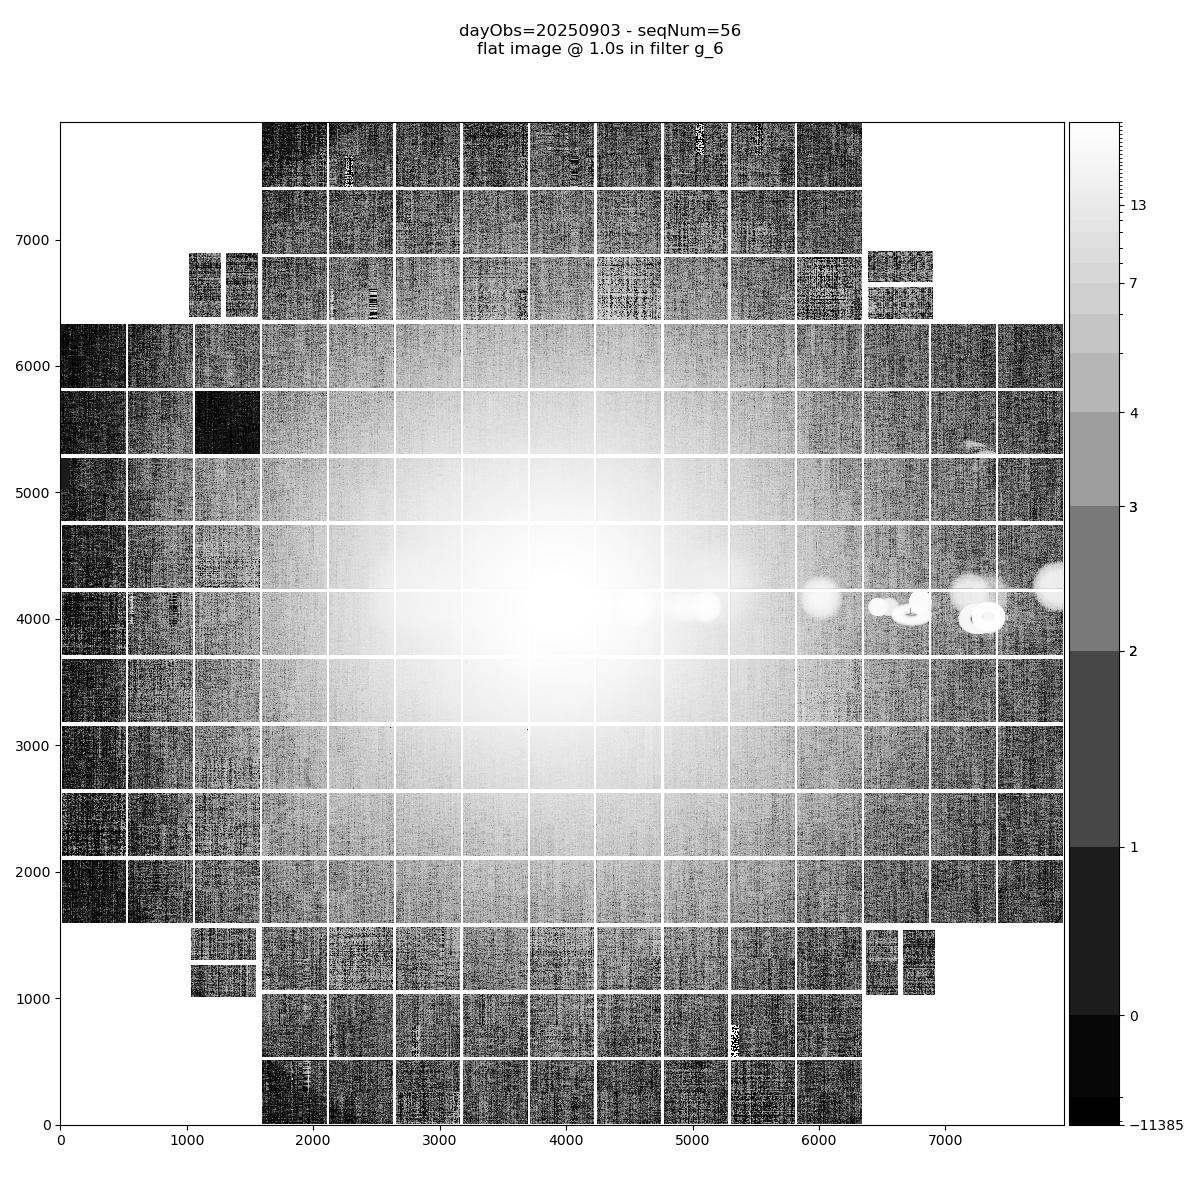
\includegraphics[width=\linewidth]{figures/cbp_ghosts_1.jpg}
    \caption{}
    \label{subfig:cbp_ghosts_a}
  \end{subfigure}
  \hfill
  \begin{subfigure}[t]{0.45\textwidth}
    \centering
    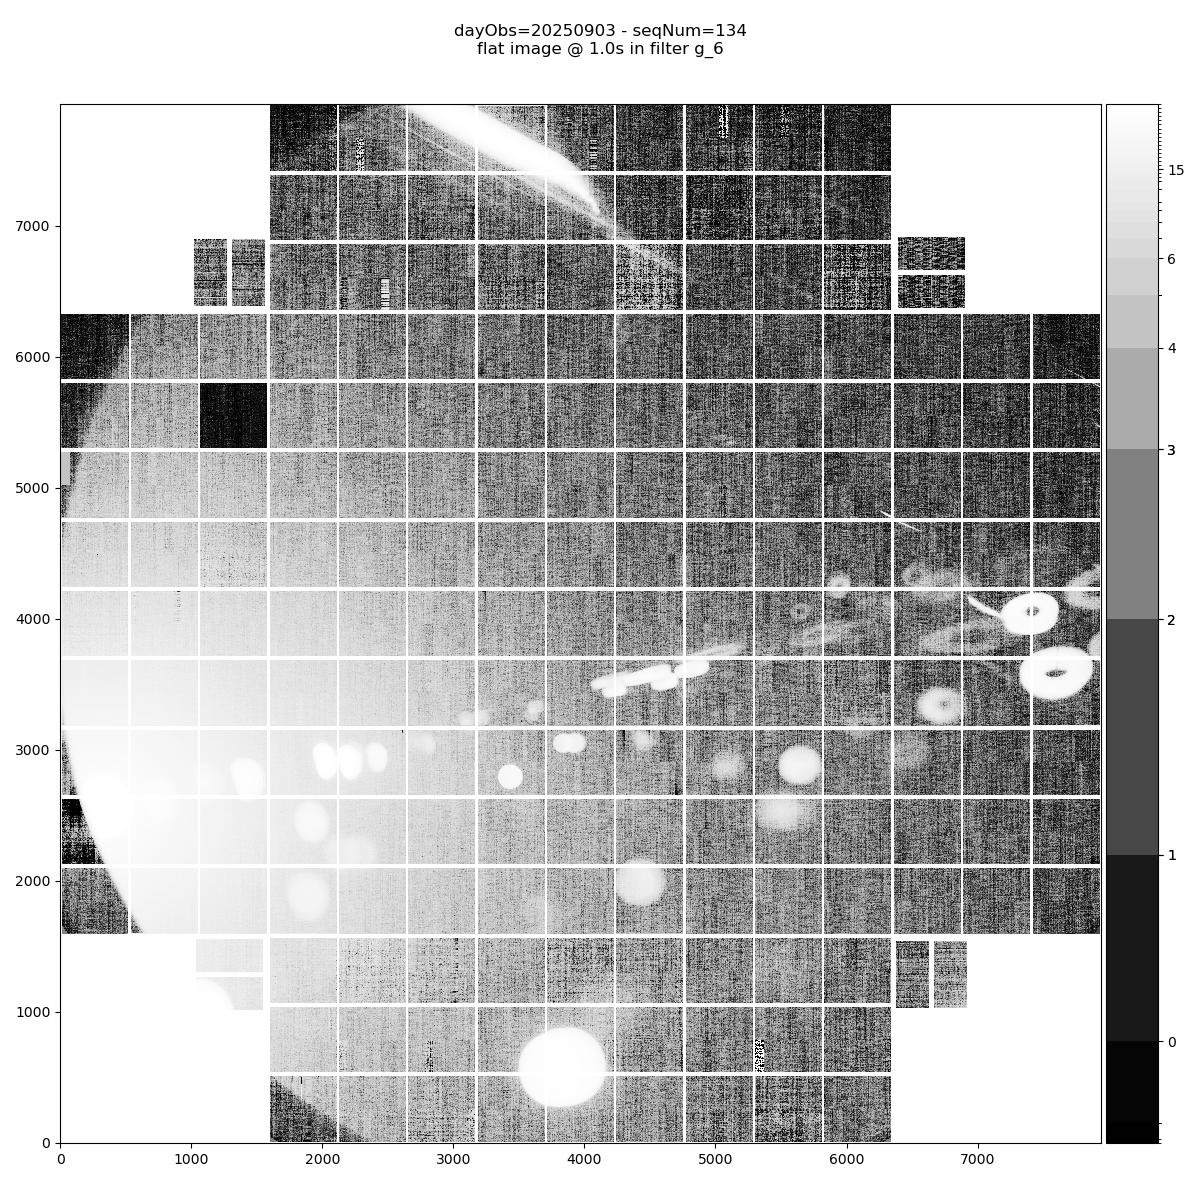
\includegraphics[width=\linewidth]{figures/cbp_ghosts_2.jpg}
    \caption{}
    \label{subfig:cbp_ghosts_b}
  \end{subfigure}

  \caption{Subfigures~\ref{subfig:cbp_ghosts_a} and \ref{subfig:cbp_ghosts_b} show the ghosts produced by a single spot CBP beam at two different pointings of the CBP in the {\it g} band.}
  \label{fig:cbp_ghosts}
\end{figure}

Figure~\ref{fig:cbp_ghosts} shows two examples of the CBP ghost data collected at various CBP-TMA pointings in the \textit{g} band.
We use the CBP to generate optical ghosts on the focal plane to avoid the challenges associated with on-sky data, including sky background fitting and crowded stellar fields.
Furthermore, the flexibility in the CBP--TMA pointing configuration allows us to generated ghosts that are more spatially separated than those that come from on-axis, on-sky data (cf. Figs.~\ref{fig:optical_ghosts} and \ref{fig:cbp_ghosts}).

Our data was collected during one CBP run performed during Rubin Observatory commissioning on 2025-09-03.
Our data taking configuration involved sweeping the CBP leftward (toward $-X$ in focal plane coordinates) starting from the center of the focal plane. 
We collected 36 images with `no filter' (519\,nm), 36 images in \textit{g} band (520\,nm), 18 in \textit{r} band (620\,nm) and 7 in \textit{i} band (760\,nm) (visit numbers 2025090300038 to 2025090300134).

\subsubsection{Ghost Flux Fitting}
\label{sec:ghost_fit}

\begin{figure}[h!]
  \centering

  \begin{subfigure}[t]{0.54\textwidth}
    \centering
    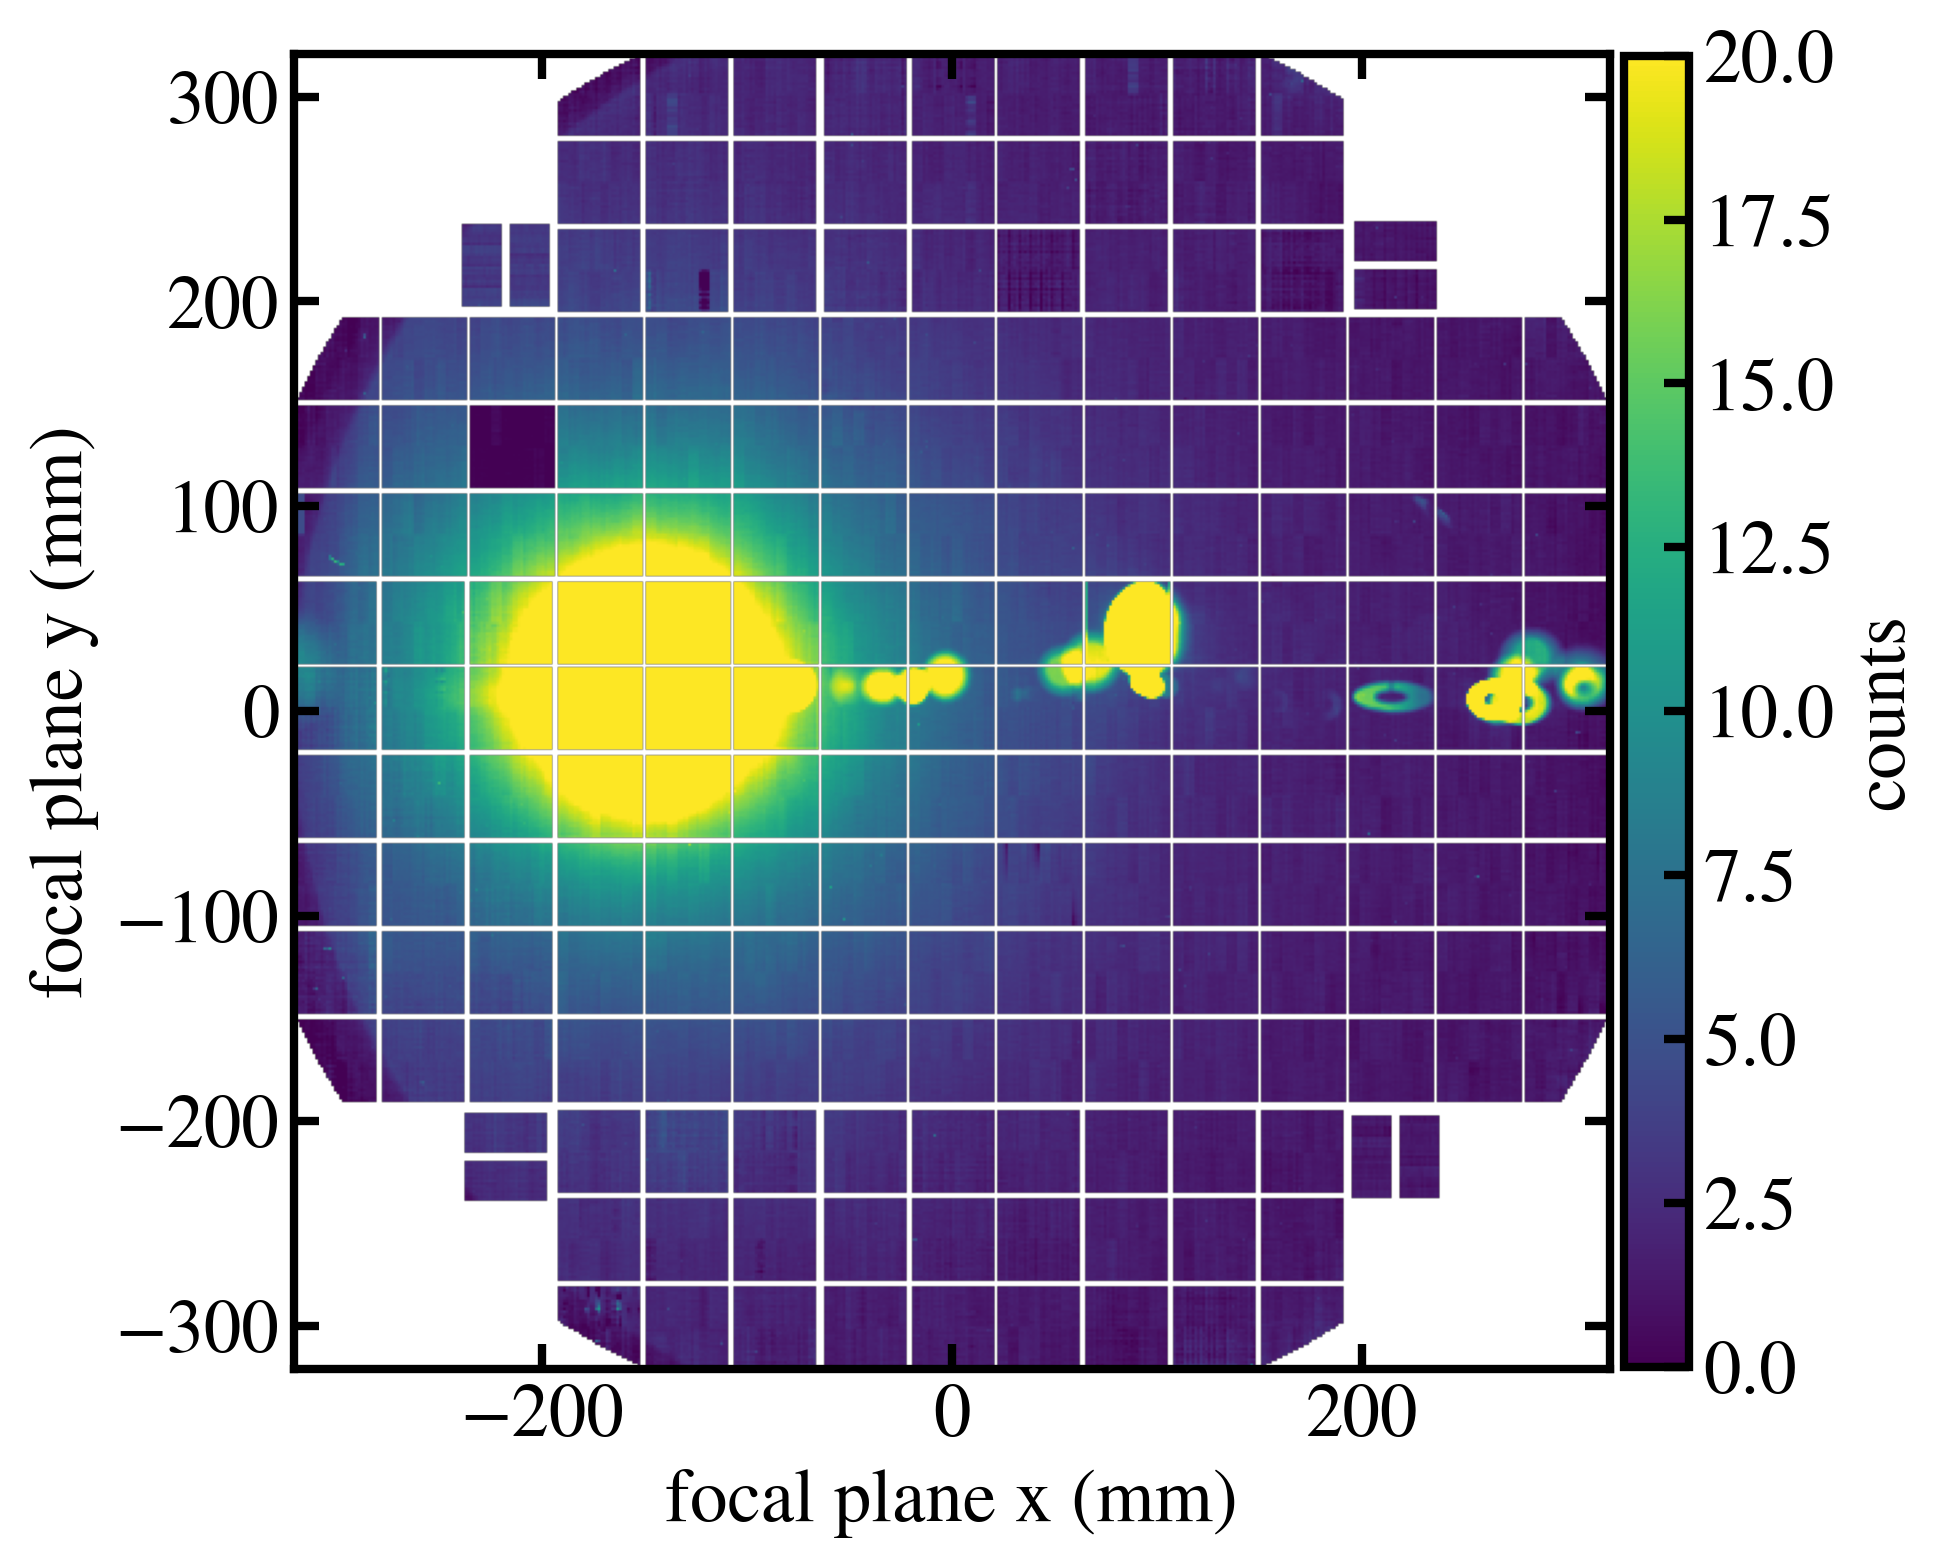
\includegraphics[width=\linewidth]{figures/CBP_ghost_data.png}
    \caption{}
    \label{subfig:cbp_data}
  \end{subfigure}
  \hfill
  \begin{subfigure}[t]{0.45\textwidth}
    \centering
    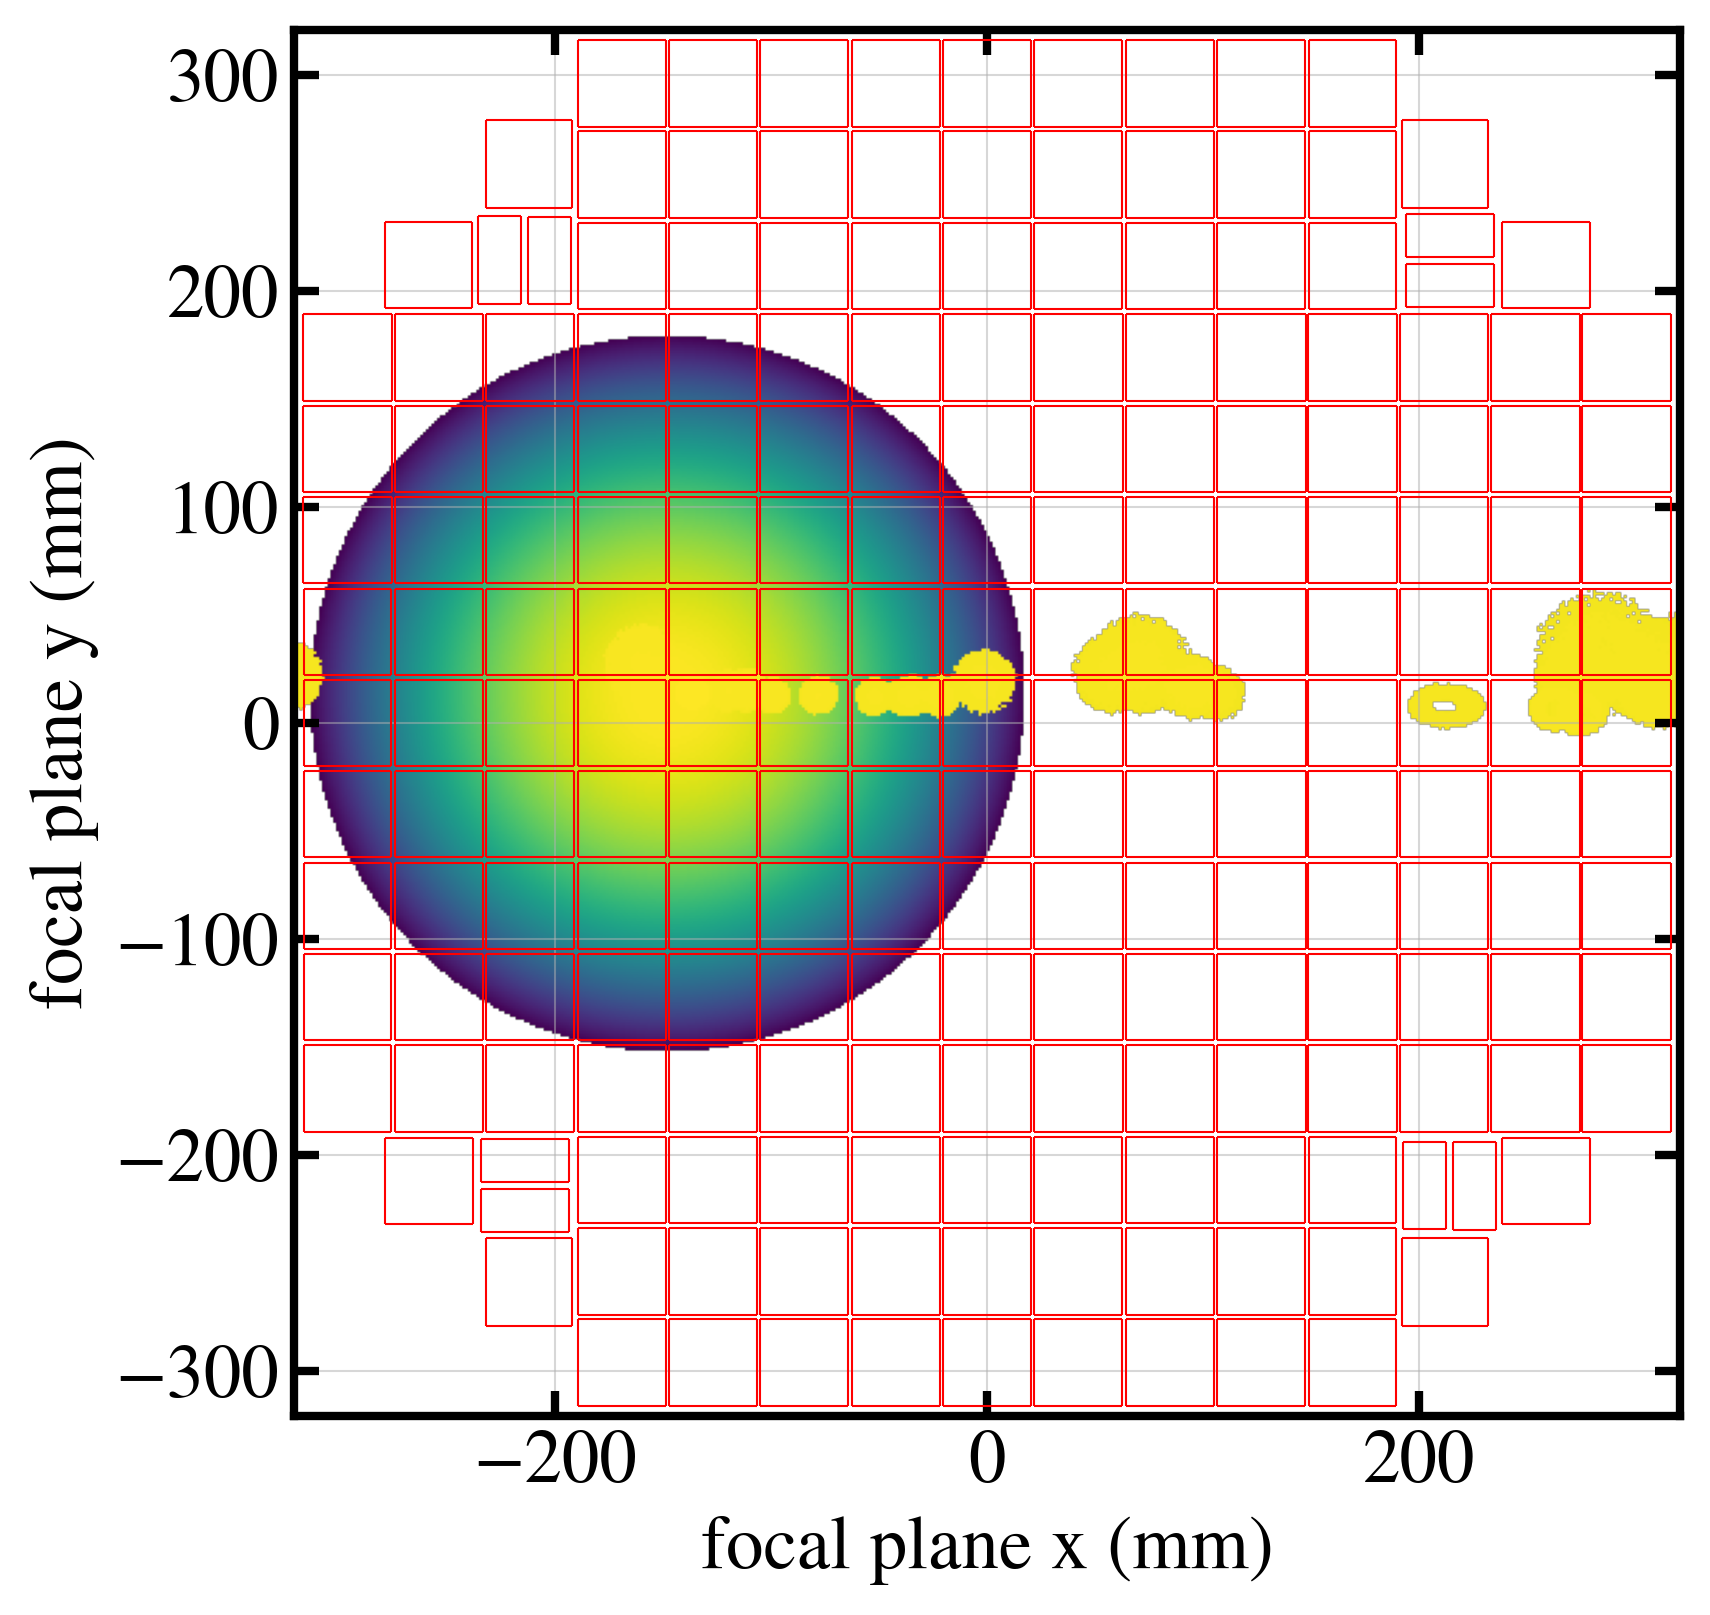
\includegraphics[width=\linewidth]{figures/CBP_ghost_sim.png}
    \caption{}
    \label{subfig:cbp_sim}
  \end{subfigure}

  \caption{The left panel shows an example of a CBP ghost image (visit 2025090300060) in {\it g} band. 
  Note that the colour bar is clipped to show the faint ghosts; the source beam is on the order of $10^5$ counts. 
  The right panel shows the CBP ghosts simulated in \texttt{Batoid} along with the Gaussian template, all normalized to 1.}
  
  \label{fig:cbp_ghost_templates}
\end{figure}

We bin the data collected from the CBP into images of 494 $\times$ 493 pixels.
We use \texttt{Batoid} to generate templates of the CBP ghosts using its built-in CBP model. 
Each simulated ghost is binned with the same resolution as the data, and then the template is normalized to have a maximum amplitude of 1.
We also include a constant background template.
Finally, we use a flat-top Gaussian model as described in Eq.~\ref{eq:flat_gaussian} to account for the saturated source beam.
Here, $r_0$ is the radius within which the Gaussian is "saturated" at amplitude $A$.
We use a radial average of the data (centered at the beam location on the focal plane retrieved from \texttt{Batoid}) to determine the width and amplitude of the Gaussian model.
The background and Gaussian templates are also normalized to a maximum value of 1.
We find that the following 16 ghosts originating from the detectors (D), filter (F), and lenses (L1, L2, L3) are the most prominent: L12-L11, L22-L11, L22-L12, F2-L21, F1-L21, F1-L22, L32-L22, L31-L22, D-L22, D-F1, D-F2, D-L31, L31-F2, L32-F1, L32-F2, L31-F1.
Figure~\ref{fig:cbp_ghost_templates} shows an example of the binned data and the 16 ghost templates and the Gaussian template simulated in \texttt{Batoid}.

\begin{equation}
\label{eq:flat_gaussian}
f(r) =
\begin{cases}
A, & r \le r_0 \\
A \exp\left(-\dfrac{(r - r_0)^2}{2\sigma^2}\right), & r > r_0
\end{cases}
\end{equation}

We then use non-negative least squares to fit the data twice. 
\begin{enumerate}
\item In the first fit, we use all the normalized templates (ghosts, background, and Gaussian) to measure the amplitude of each prominent ghost.
\item In the second fit, since the saturated source flux is orders of magnitude larger than the ghosts, we mask the region occupied by the Gaussian template and fit only the CBP ghosts and background to ensure that the fits are not skewed due to the source fit.
\end{enumerate}

\subsection{Reflectance Measurements}
After measuring the fluxes of the CBP ghosts, we measure the reflectances of the telescope optics using Eq.~\ref{eq:reflectance_matrix} in Sec.~\ref{sec:reflectance_theory}. 
Figure~\ref{fig:reflectance_vs_optic} shows the reflectances of each optical element in the no-filter (labelled ``None'') and {\it g}, {\it r}, and {\it i} bands.
Note that measurements for F1, F2 and L21 are not available in the no-filter data (the latter is unavailable as the most prominent ghosts from L21 also require the filter).
More detailed distributions of the reflectance measurements (with both the fit to the source and without are shown in Appendix~\ref{app:reflectance_hists}.

\begin{figure}[h!]
    \centering
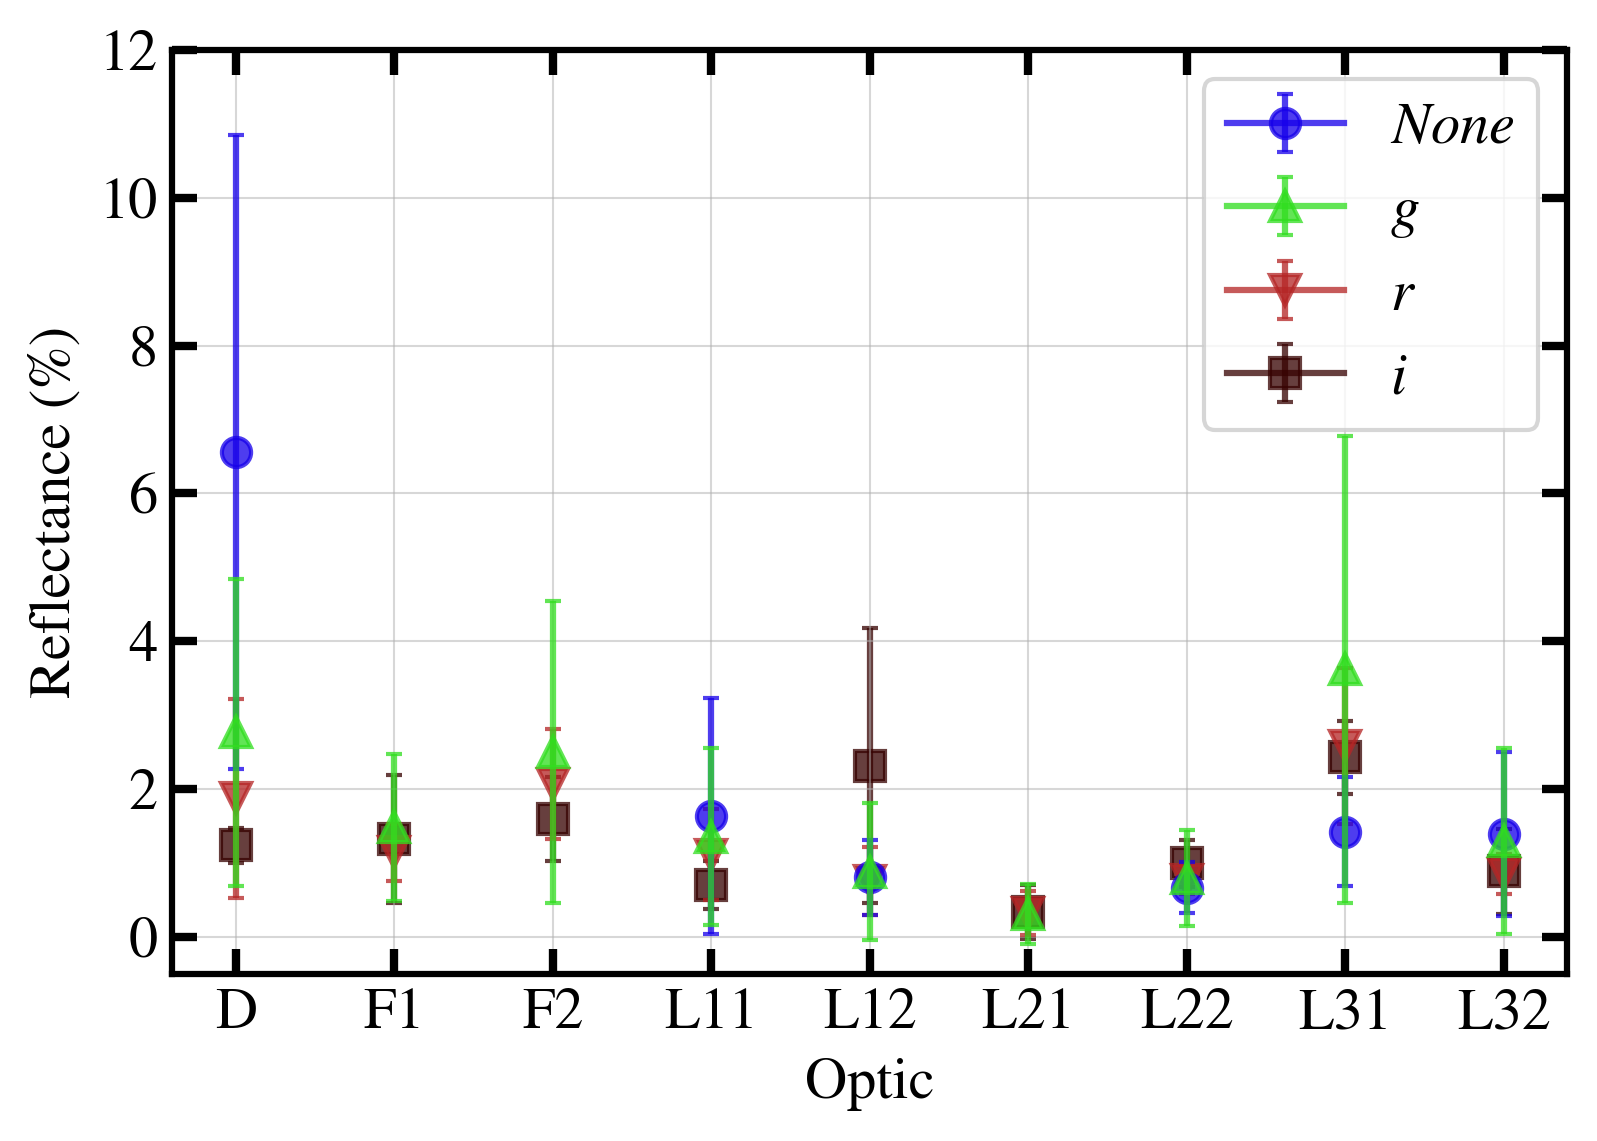
\includegraphics[width=0.75\textwidth]{figures/reflectance_vs_optic.png}
    \caption{Measured reflectances for each optical surface. The measurements are made at a single wavelength for each optical configuration: no-filter (519\,nm), {\it g} (520\,nm), {\it r} (620\,nm), and {\it i} (760\,nm).} 
    \label{fig:reflectance_vs_optic}
\end{figure}
 Table~\ref{tab:syseng_throughputs} shows the simulated reflectance values for the detector and filter (F$_s$ \& D$_s$) produced by the systems engineering simulations. Note that these simulations do not differentiate the two surfaces of the optical elements. The table also contains our measured F1, F2 and D reflectances derived from the masked-source fits and the wavelengths of the laser that we used to produce the CBP ghosts in each band.

\begin{table}[t!]
\centering
\begin{tabular}{cccccccc}
\hline
Band & Wavelength (nm) & F$_s$ (\%) & D$_s$ (\%) & F1 (\%) & F2 (\%) & D (\%) \\
\hline
$None$ & 519 & N/A & 6.84 & N/A & N/A & 6.56 $\pm$ 4.29 \\
$g$ & 520 & 2.52 & 6.79 & 1.48 $\pm$ 0.99 & 2.50 $\pm$ 2.04 & 2.77 $\pm$ 2.08\\
$r$ & 620 & 3.89 & 2.98 & 1.14 $\pm$ 0.38 & 2.07 $\pm$ 0.74 & 1.87 $\pm$ 1.35\\
$i$ & 760 & 1.54 & 4.15 & 1.32 $\pm$ 0.86 & 1.59 $\pm$ 0.57 & 1.24 $\pm$ 0.24\\
\hline
\end{tabular}
\caption{Systems engineering optical reflectances (F$_s$ \& D$_s$) and our measurements (F1, F2 \& D) for the filter and detector.}
\label{tab:syseng_throughputs}
\end{table}

 We observe that our measurements of the reflectances of the detector and filter are around the 2\% level.
 We also observe that the measurements of the reflectances with and without masking the source are consistent with each other, leading us to believe that the fit of the source beam is not skewing the measured reflectances.
 The large error bar in the measurement of the reflectance of the detector in the no-filter setting is due to the fact that the most significant ghosts produced by the detector are the D-F1 and D-F2 ghosts, which are absent when the filter is not present, thus reducing the constraining power of the model.